\subsubsection{UC8.3 - Personalizzazione Force Field}
\begin{figure}[h]
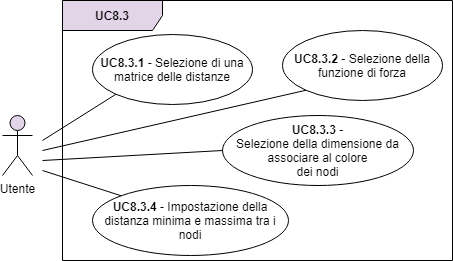
\includegraphics[width=14cm]{Section/Images/UC8.3.png}
\centering
\caption{UC6.3 - Personalizzazione Force Field}
\end{figure}
\begin{itemize}
	\item \textbf{Attore primario}: Utente;
	
	\item \textbf{Precondizioni}: L'utente ha scelto il grafico \textit{Force Field} [UC7.2];
	
	\item \textbf{Postcondizioni}: Il grafico viene aggiornato;
	
	\item \textbf{Scenario principale}: L'utente decide:
	
\begin{enumerate}
\item Una matrice delle distanze calcolata in precedenza [UC8.3.1];
\item Il tipo di funzione di forza [UC8.3.2];
\item La dimensione d'associare al colore dei nodi [UC8.3.3];
\item La distanza minima e massima tra i nodi [UC8.3.4].
\end{enumerate}	
		
\end{itemize}

